%\begingroup
%\setsecnumdepth{part} 
\chapter{Konklusion} 
\label{chap:konklusion}
\thispagestyle{empty}

Vores mål med dette speciale var at undersøge muligheden for en udvidelse af \pycsp, der muliggør brugen af tid direkte i sproget. Der findes allerede et massivt teoretisk arbejde inden for området, men ingen praktisk anvendelige implementeringer, så vores fokus har været på, at det skulle være praktisk anvendeligt. Dette afspejles i, at vi har valgt at benytte eksempler som omdrejningspunkt for vores analyser af de tre anvendelsesområder. 

De tre anvendelsesområder vi identificerede i introduktionen var diskret simulering, realtidsplanlægning og interaktiv planlægning. Vi har vha. analyser af krav og eksempler udviklet løsninger der imødekommer alle tre amvendelsesområder. 

Inden for diskret simulering har vi udviklet en løsning, der er let at anvende, og som eliminerer kravet om en delt datastruktur for at administrere tid i \pycsp. Dette er gjort ved at introducere en repræsentation af tid i skemaplanlæggeren, samt styring af aktivering af processer ud fra denne tid. Løsningen er let at anvende og kræver væsentligt mindre kode til at administrere tiden, end en tilsvarende løsning lavet i ren \pycsp. 
Sammenligner vi vores løsning med \simpy, der er et framework til simuleringer, skrevet i Python, mener vi at vores løsning er mere intuitiv og fleksibel at benytte til at modellere et givet problem. Dette skyldes i høj grad, at vi direkte kan benytte \pycsp's processer og kanaler. Et eksempel på hvordan diskret simulering i \pycsp giver udvikleren større frihed til sin modellering finder vi i en kommende udvidelser til \simpy. Der arbejdes  på at udvide \simpy til at kunne håndtere reservation af flere begrænsede ressourser, som skal benyttes samtidigt. Dette er allerede muligt i vores løsning, uden det har været vores fokus, da ressourcer blot modelleres som processer i \pycsp. Ønsker man at reservere flere ressourcer, kommunikerer man blot med flere processer, og når alle processerne har svaret, holder man alle de begrænsede resourcer. Arbejdet kan nu udføres, og ressourcerne frigives igen. 

I vores løsning til realtidsplanlægning har vi udvalgt earliest deadline first (EDF), som den grundlæggende skemaplanlægningsalgoritme til at bestemme rækkefølgen for udførsel af processer. Vi har implementeret prioritetsnedarvning for at imødekomme problemer med prioritetsinvertering samt indført en prioriteret udvælgelse i \code{alternations}, og når der kommunikeres over kanaler. Vores eksempel viser tydeligt, at vores løsning vha. af planlægning, kan øge effektiviteten, såfremt der i programmet kan foretages en differentiering i prioriteten af de processer, der skal afvikles. 

Vi er kommet frem til, at interaktiv planlægning ikke kan anses som et selvstændigt anvendelsesområde, men nærmere som en gren af realtidsplanlægning. De benytter begge realtid som tidsmodel, og har begge deadlines og prioriteter. Interaktiv planlægning gør det lettere at udtrykke et starttidspunkt vha. venten, men er ellers ikke fundamentalt forskellig fra realtidsplanlægning. Vi mener derfor at det er mere hensigtsmæssigt at anskue anvendelsesområderne ud fra hvilken tidsmodel, de bygger på. \CRef{fig:timemodel} viser således opdelingen af anvendelsesområderne i henholdsvis diskret og realtid.

\begin{figure}[htp]
 \begin{center}
  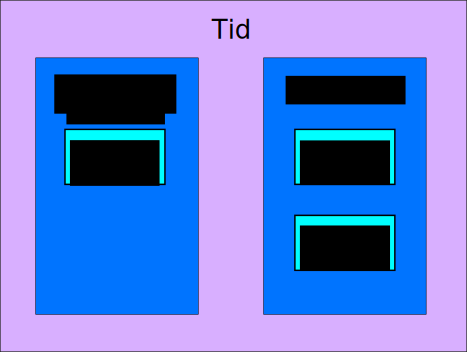
\includegraphics[scale=0.6]{images/timemodel}
	\caption{Forholdet mellem de tre anvendelsesområder vi opstillede i introduktionen.}
	\label{fig:timemodel}
\end{center}
\end{figure}


Vi har gennem vores eksempler, vist at vores løsninger er brugbare i den nuværende form, men der kan foretages en række udvidelser, der vil gøre dem endnu mere anvendelige. 
Inden for diskret simulering synes vi det kunne være spændende at udvide løsningen til at kunne foretage en dynamisk evaluering af køer, for derved at give ekstra fleksibilitet i de udviklede simuleringer. I realtidsplanlægning har vi lavet en basisimplementering, der benytter EDF. Det kunne være interessant at kigge på mulighederne for at bedømme en proces' udførselstid, eller lade udvikleren angive dette. Herved åbnes op for brug af adskillige andre algoritmer end EDF til skemaplanlægningen og udvider anvendelsesområdet.  

%lettere at modellere processer
%Simpy kan ikke reservere begrænsede ressourcer

%Sammenligning med Simpy her 

%Tidsmodeller/anvendelsesområder

%Praktisk anvendelig implementering

%nuværende tilstand for anvendelsesområderne

%\endgroup 

